\section{Zustandsbasierte Systeme}

\subsection{Asynchrone vs. synchrone FSM}

\begin{minipage}[t]{0.48\columnwidth}
    \raggedright
    \begin{outline}
        \1 \textbf{Asynchron}
            \2 geänderte Inputsignale führen \textbf{direkt} zur Zustandsänderung
            \2 schneller, aber enorm anfällig auf Glitches
    \end{outline}
\end{minipage}
\hfill
\begin{minipage}[t]{0.48\columnwidth}
    \raggedright
    \begin{outline}
        \1 \textbf{Synchron}
            \2 Inputsignale werden nur zu diskreten Zeitpunkten betrachtet \\
                \textrightarrow\ getaktete Systeme
    \end{outline}
\end{minipage}

\vspace{0.2cm}

\begin{outline}
    \1 Softwareimplementationen sind eigentlich immer \textbf{synchron}, da Rechner getaktet sind
    \1 Rein softwareseitig besteht die Problematik der Asynchronizität nicht
\end{outline}


\subsection{Finite State Machines (FSM)}

\begin{center}
    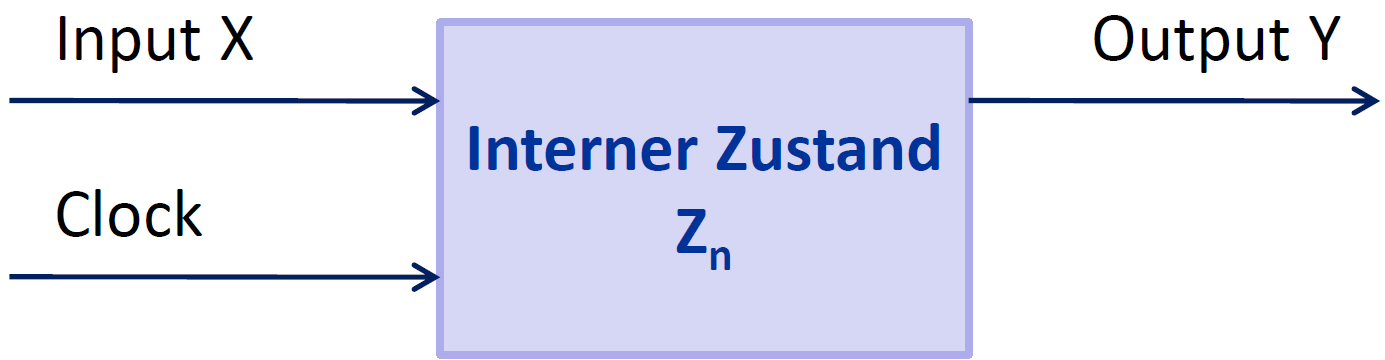
\includegraphics[width=0.7\columnwidth]{images/fsm.png}
\end{center}

Eine FSM besitzt die folgenden Eigenschaften:

\vspace{0.1cm}

\begin{outline}
    \1 Eine FSM befindet sich immer in einem \textbf{definierten Zustand}
    \1 Die \textbf{Inputs} $X$ bezeichnen üblicherweise \textbf{Ereignisse (Events)}
    \1 Die \textbf{Outputs} $Y$ werden oft auch \textbf{Actions} genannt
    \1 Eine FSM benötigt immer \textbf{Speicherelemente} zur Speicherung des internen Zustands
        \2 Eine FSM ist ein sequenzielles und kein kombinatorisches System
\end{outline}

\vspace{0.2cm}

Eine FSM kann auf zwei Arten dargestellt werden:

\vspace{0.1cm}

\begin{minipage}[t]{0.48\columnwidth}
    \begin{itemize}
        \item State-Event-Diagramm
    \end{itemize}
\end{minipage}
\hfill
\begin{minipage}[t]{0.48\columnwidth}
    \begin{itemize}
        \item Zustandstabelle
    \end{itemize}
\end{minipage}


\subsubsection{Mealy-Automat}

\begin{outline}
    \1 Nächster Zustand $Z_{n+1}$ abhängig vom Input $X$ und vom internen Zustand $Z_n$
        \2 $Z_{n+1} = f(Z_n, \, X)$
    \1 Output $Y$ ist abhängig vom internen Zustand $Z_n$ \textbf{\crd{und vom Input $X$}}
        \2 $Y = g(Z_n , \, X)$
    \1 Actions liegen bei den Transitionen
\end{outline}


\subsubsection{Moore-Automat}

\begin{outline}
    \1 Nächster Zustand $Z_{n+1}$ abhängig vom Input $X$ und vom internen Zustand $Z_n$
        \2 $Z_{n+1} = f(Z_n, \, X)$
    \1 Output $Y$ ist \textbf{\crd{nur}} abhängig vom internen Zustand $Z_n$ 
        \2 $Y = g(Z_n)$
    \1 Actions liegen bei den Zuständen
\end{outline}

\vspace{0.1cm}

\textbf{ \textrightarrow\ Wenn immer möglich sollten Moore-Automaten verwendet werden}

% CHECK: könnte man auch entfernen...
\subsubsection{Medvedev-Automat}

\begin{outline}
    \1 Nächster Zustand $Z_{n+1}$ abhängig vom Input $X$ und vom internen Zustand $Z_n$
        \2 $Z_{n+1} = f(Z_n, \, X)$
    \1 Output $Y$ entspricht \textbf{entspricht direkt} internem Zustand $Z_n$ 
        \2 $Y = Z_n$
    \1 Actions liegen bei den Zuständen
\end{outline}

\vspace{0.1cm}

\textrightarrow\ Wird hier nicht weiter behandelt...


\subsection{State-Event-Diagramm (Zustandsdiagramm)}

Ein State-Event-Diagramm ist eine grafische Möglichkeit, um eine FSM zu beschreiben. \\
In einem State-Event-Diagramm gelten folgende Darstellungsformen    % CHECK besseres Wort als 'Darstellungsformen'?

\vspace{0.1cm}

\begin{itemize}
    \item \textbf{Zustände} werden mit einem \textbf{Kreis} gezeichnet
    \item \textbf{Ereignisse} werden mit \textbf{Pfeilen} zwischen Zuständen dargestellt \textbf{(Transitionen)}
    \item \textbf{Aktionen} werden entweder bei Zuständen oder bei Transitionen geschrieben (je nach Automatentyp)
    \item Ausführung einer Transition ist unendlich schneller \\
        \textrightarrow\ Bei Modellierung sind Zwischenzustäde vorgehesen, z.B. 'closing', starting up'
\end{itemize}


\example{State-Event-Diagramm -- Moore Automat}

\begin{center}
    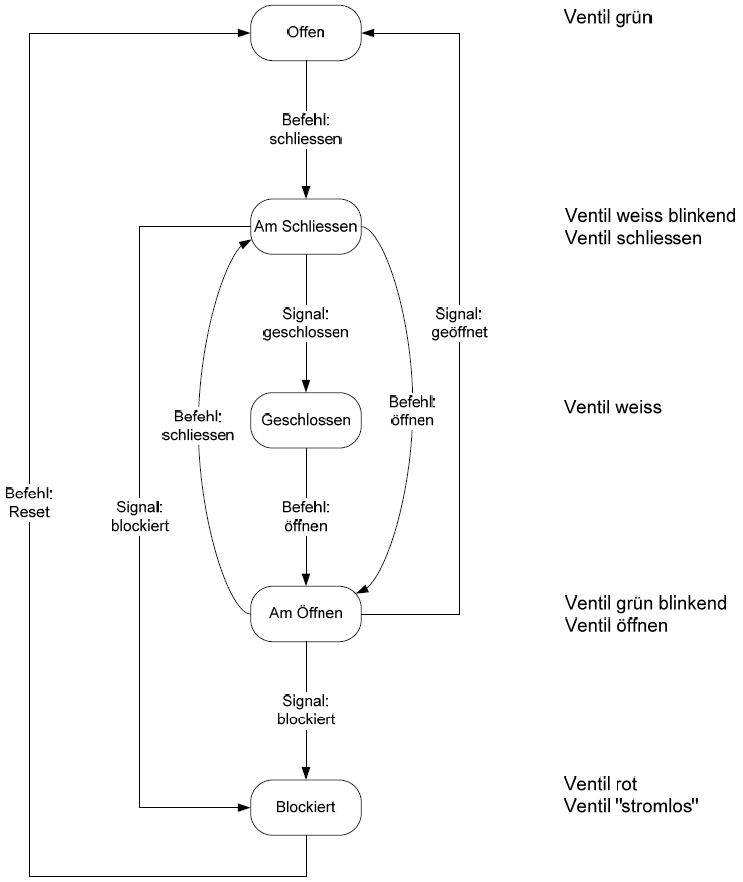
\includegraphics[width=0.8\columnwidth]{images/state_event_example.png}
\end{center}


\subsection{Zustandstabelle}

Nebst der grafischen Darstellung einer FSM mittels State-Event-Diagramm kann die FSM auch tabellarisch mittels Zustandstabelle 
beschrieben werden.


\example{Zustandstabelle für Elektromotor}

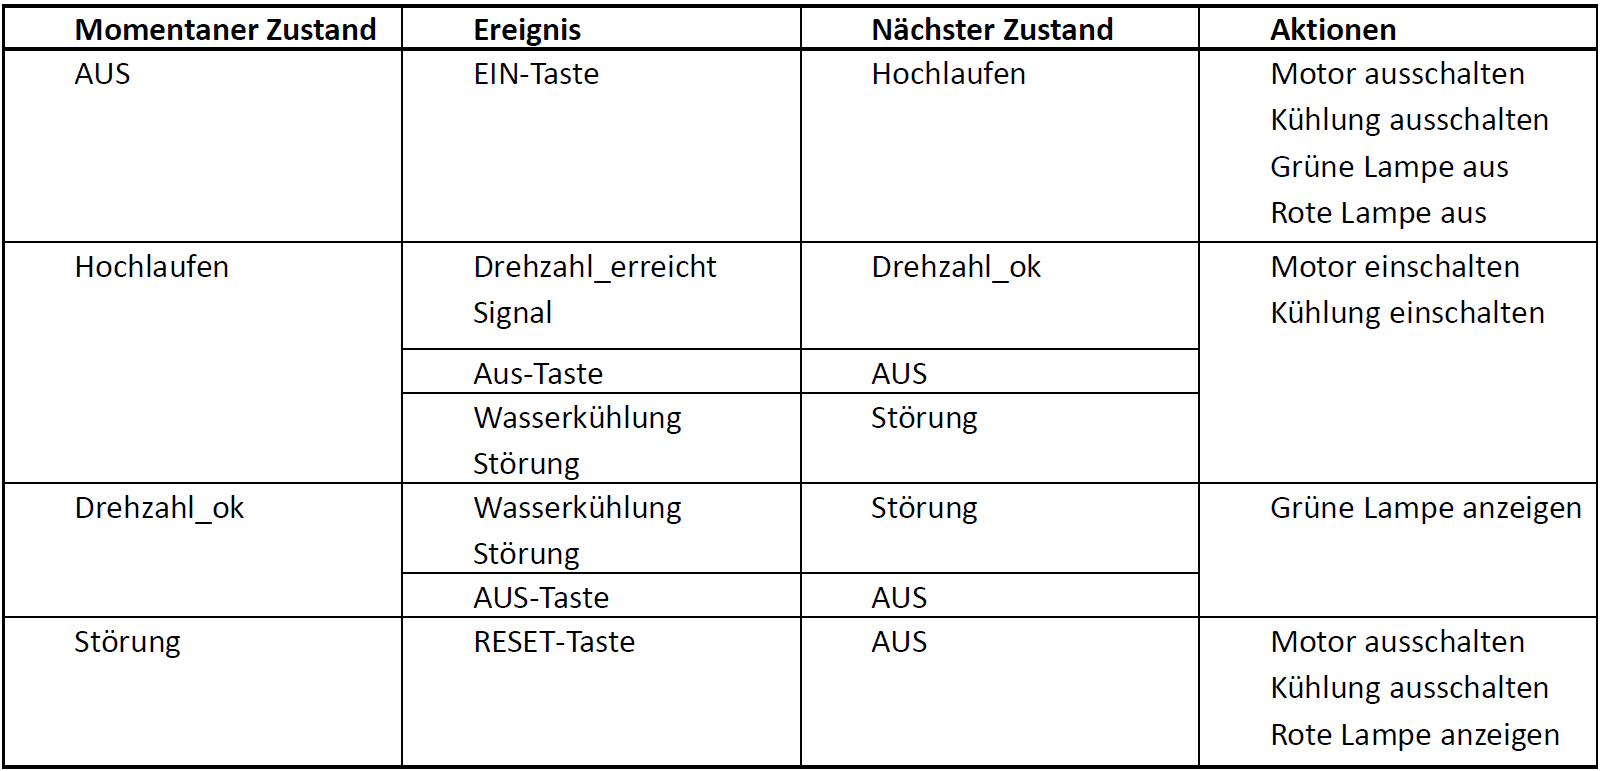
\includegraphics[width=\columnwidth]{images/zustandstabelle.png}